\documentclass[english]{exam}

\setlength {\marginparwidth }{2cm} 
\usepackage{todonotes}

\usepackage[perpage,para,symbol]{footmisc}

\hyphenpenalty=15000 
\tolerance=1000

\usepackage{tikz}
\usetikzlibrary{arrows,decorations.pathmorphing,backgrounds,fit,positioning,calc,shapes}
\usepackage{pgfmath}
\usepackage{rotating}
\usepackage{array}	
\usepackage{graphicx}
\usepackage{float}	
\usepackage{mdwlist}
\usepackage{setspace}
\usepackage{listings}
\usepackage{bytefield}
\usepackage{tabularx}
\usepackage{multirow}	       
\usepackage{caption}
\usepackage{amssymb}
\captionsetup[table]{skip=10pt}

\usepackage{url}               
\usepackage{hyperref}
\usepackage[all]{hypcap}	
\usepackage{titlesec}
\setcounter{secnumdepth}{4}
\titleformat{\paragraph}
{\normalfont\normalsize\bfseries}{\theparagraph}{1em}{}
\titlespacing*{\paragraph}
{0pt}{3.25ex plus 1ex minus .2ex}{1.5ex plus .2ex}
\hypersetup{colorlinks,breaklinks,
            linkcolor=darkblue,urlcolor=darkblue,
            anchorcolor=darkblue,citecolor=darkblue}


\definecolor{darkblue}{rgb}{0.0,0.0,0.3} 
\definecolor{darkred}{rgb}{0.4,0.0,0.0}
\definecolor{red}{rgb}{0.7,0.0,0.0}
\definecolor{lightgrey}{rgb}{0.8,0.8,0.8} 
\definecolor{grey}{rgb}{0.6,0.6,0.6}
\definecolor{darkgrey}{rgb}{0.4,0.4,0.4}
\definecolor{aqua}{rgb}{0.0, 1.0, 1.0}
\definecolor{dkgreen}{rgb}{0,0.6,0}
\definecolor{gray}{rgb}{0.5,0.5,0.5}
\definecolor{mauve}{rgb}{0.58,0,0.82}

\lstset{
  language=C,
  showstringspaces=false,
  columns=flexible,
  basicstyle={\small\ttfamily},
  numbers=none,
  numberstyle=\tiny\color{gray},
  keywordstyle=\color{blue},
  commentstyle=\color{dkgreen},
  stringstyle=\color{mauve},
  breaklines=true,
  breakatwhitespace=true,
  tabsize=3
}

\definecolor{mGreen}{rgb}{0,0.6,0}
\definecolor{darkblue}{rgb}{0.1,0.1,0.5}
\definecolor{mGray}{rgb}{0.5,0.5,0.5}
\definecolor{mPurple}{rgb}{0.58,0,0.82}
\definecolor{backgroundColour}{rgb}{0.95,0.95,0.92}

\hypersetup{colorlinks,breaklinks,
            linkcolor=darkblue,urlcolor=darkblue,
            anchorcolor=darkblue,citecolor=darkblue}


\lstdefinestyle{CStyle}{
    backgroundcolor=\color{backgroundColour},   
    commentstyle=\color{mGreen},
    keywordstyle=\color{magenta},
    numberstyle=\tiny\color{mGray},
    stringstyle=\color{mPurple},
    basicstyle=\footnotesize,
    breakatwhitespace=false,         
    breaklines=true,                 
    captionpos=b,                    
    keepspaces=true,                 
    numbers=left,                    
    numbersep=5pt,                  
    showspaces=false,                
    showstringspaces=false,
    showtabs=false,                  
    tabsize=2,
    language=C
}

\usepackage{listings}
\PassOptionsToPackage{USenglish,english}{babel} 
\usepackage{csquotes}
\usepackage[USenglish,english]{babel}
\usepackage[acronym, section=section, nonumberlist, nomain, nopostdot]{glossaries}
\makeglossaries
 
\makeglossaries
\newcommand{\colorbitbox}[3]{%
	\rlap{\bitbox{#2}{\color{#1}\rule{\width}{\height}}}%
	\bitbox{#2}{#3}}

\begin{document}

\title{Project Report: \\ The Ray Tracing Model}
\author{Calin Capitanu}

\maketitle
\begin{center}
  \url{https://github.com/capitanu/DD2360} \\
\end{center}

\section*{Introduction}

Ray tracing is a common problem when it comes to parallelization. The idea behind ray tracing is to have objects in a scene, a camera, a canvas and some light sources. From there on, most of the part is just a lot of computation, which is done as following: there are drawn lines from the camera through each pixel on the canvas, checked for intersections with the object, and if that is the case, applied some ``filters'' for light, reflection and so on.
\\\\
The interesting part here, however, is the fact that every ray that goes from the camera through the canvas is completely independent of the others, thus, it makes of a really good application for GPU, besides the obvious reason that there are a lot of pixels for which this needs to be computer, which once again, GPUs are good at (small but lots of computations).
\\\\
Each pixel that I trace a ray through has to find whether or not the trace will intersect the object at hand, and if not, the pixel should be empty (or black), otherwise, we need to do more computations in order to figure out the lights, shadows and reflections. \cite{ray-1}

\section*{Methodology}

The first steps that I took in order to solve this assignment was to refresh my memory on how exactly Ray-Tracing works. The tutorial and python code supplied online was really helpful in this sense, and also for further implementations.
\\\\
Once the tools used were chosen, then, the second step was to recreate the same code for ray tracing in a CUDA file that would run on the CPU, try to get similar results and time it. Python does a great job in some kind of abstractions when it comes to array manipulation, which C++ is not as capable of doing, however, there were not too many changes needed in this sense for the CUDA code.
\\\\
The next step was to decide on what is needed for a similar GPU implementation of the same code, together with parameter choices (for example threads per block an so on). This was however coded as a definition in my program since I wanted easy access to changing it later.
\\\\
Since the main point was then to output an image, the last part was to figure out how to do so in C++, which once again was a bit harder than in Python, since one needs to write all the header details and so on. For this step, online resources were used, such as the forum Stack Overflow \cite{stack}.
\\\\

\subsection*{Data Structures and Code Brief}

Since each pixel needed 3 values from 0 to 255 in order to encode all of the colors for RGB, I decided to use an array that was of size width * height * 3, where width and height are represented by properties of the image that I am rendering. I could have also used a higher dimensional array, just as the one used in Python, however, this worked just as good.
\\
One side note here is the fact that BMP images have a different encoding than the usual RGB, but instead they are BGR (Blue, Green, Red) - slight convention issues, but nothing problematic.
\\\\
Another important aspect is the fact that the kernel just needed to be started width*height times, thus, no extra kernels for each of the three colors of the kernel, since those are computed at once, inside only one instance of the kernel.
\\\\
In terms of the actual code, in order to do a quick brief if it:
\begin{enumerate}
\item A vector from the point where the camera is through the first pixel in the canvas is normalized (size 1).
\item The next part is to actually ``Trace the Ray''. This means that first I check if the ray intersects the object or not.
\item If there is some intersection, there are some predefined formulas in order to compute the diffusion, reflection and so on.
\end{enumerate}

\section*{Experimental Setup}

The GPU used for this project is an NVIDIA GeForce RTX 3080, Ampere generation. The development of the project was done using the CUDA platform in C++. The specific cuda version used is CUDA 11.4. All of the code written was compiled using $nvcc$ with the flag $-arch=sm\_80$.
\\\\
I think one other important thing to mention here is the CPU that has been used, since it is considered really powerful, which is a good reason for some of the results to be in the favor of the CPU sometimes. The CPU used is a Ryzen 9 5950X with 32 threads and running at speed from 3.4 to 4.9 GHz.
\\\\
No other specific tools were used for the development of this project, besides the obvious operating system and some text editor which should be irrelevant to this problem at hand, but the are listed here:

\begin{enumerate}
\item Operating System: GNU/Linux: 5.11.22-2-MANJARO
\item Text Editor: GNU Emacs 27.2
\end{enumerate}

\section*{Results}

In order to check that the results achieved by the GPU version of the program are valid and correct, during development, the output of the actual kernels was used in order to generate the required image, which indicated whether or not it is at least close to expected.

\begin{figure}[H]
    \centering
    \textbf{CPU rendering}\par\medskip
    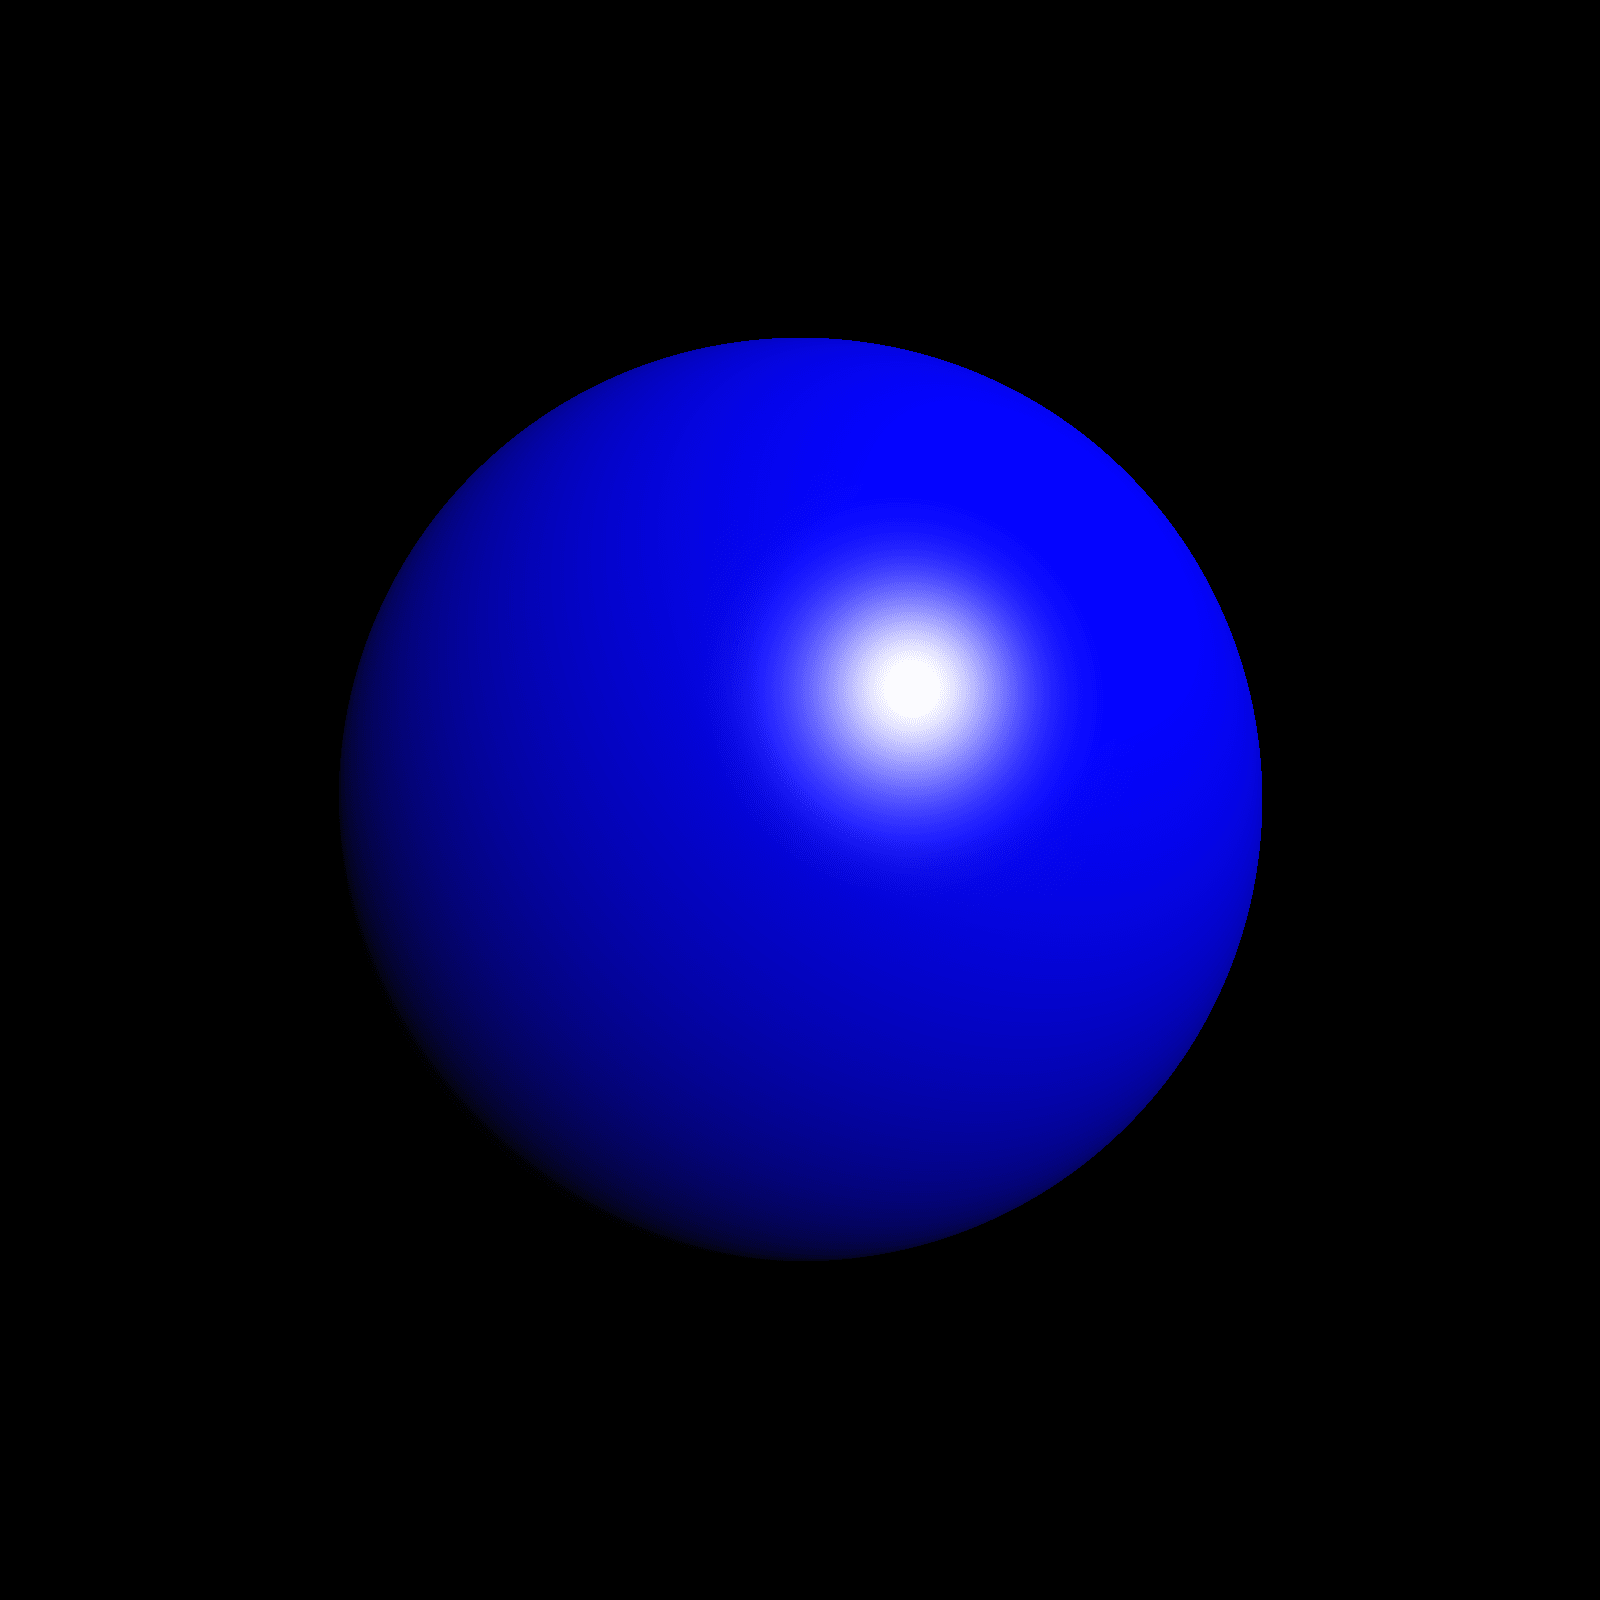
\includegraphics[scale=0.4]{cpu.png}
    \caption{}
\end{figure}
\begin{figure}[H]
    \centering
    \textbf{GPU rendering}\par\medskip
    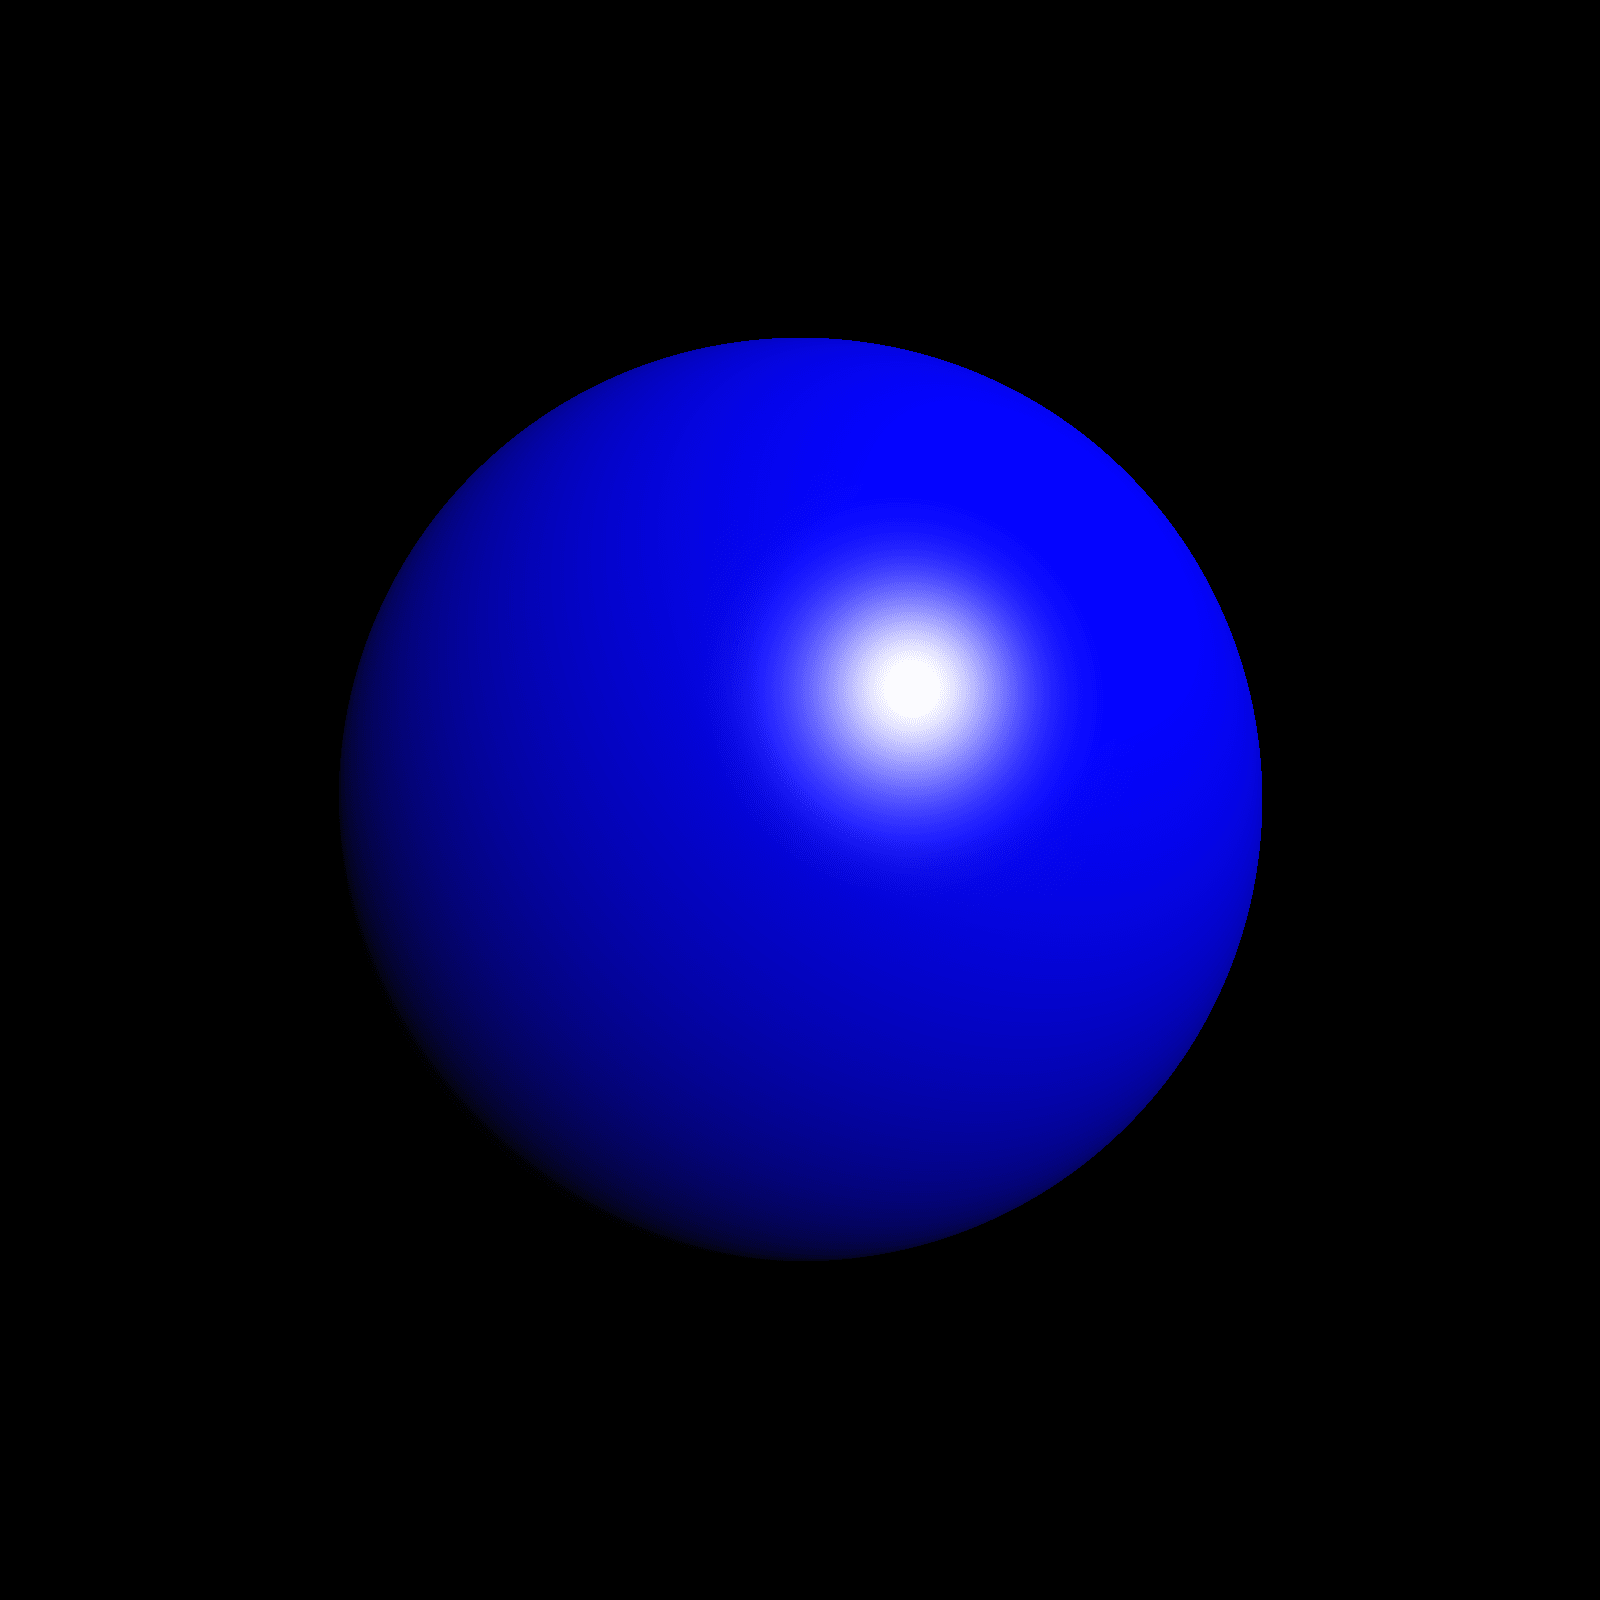
\includegraphics[scale=0.4]{gpu.png}
    \caption{}
\end{figure}


\ \\
\noindent
Once this part was done, I wanted a more ``scientific'' way of testing the results, for which I then wrote a small check function at the end in order to compare the two outputs and thus see if the error between the two exceeds some threshold. The results seem to have been equal for error rate even set to $0.01$.
\\\\
For the performance tests, I tried a couple of different value for size of the image, size of the sphere, as well as the number of threads per block in the GPU division. I chose to plot these results as well as to serve place them in a table for ease of readability, which is available in the Appendix \ref{tab:1}. The first part was to find the best configuration for the GPU number of threads per block, thus I ran it against 3 different image sizes and range of TPB from 2 to 256 (2, 4, 8, ..., 256).

\begin{center}
  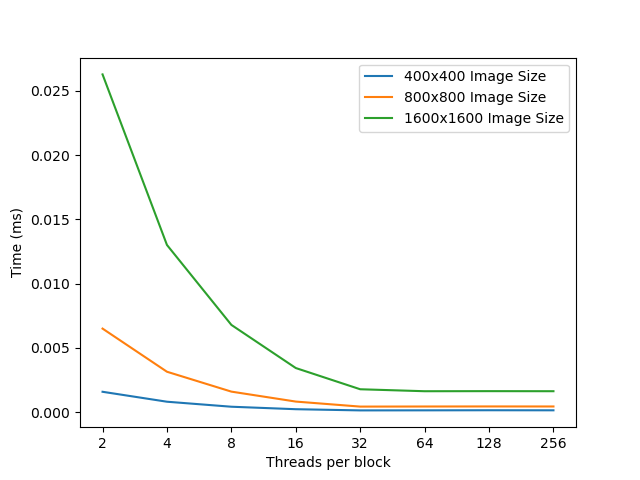
\includegraphics[scale=0.6]{plot1.png}
\end{center}


\noindent
Since the plot and table above show that the best configuration is the one with 32 threads per blocks, for the rest of the research I have only used 32 threads per block for the GPU version and started plotting different graphs for the comparison between the GPU and the CPU version of the program.
\\\\
For the next experiment, I plotted different image sizes for the GPU and the CPU. These results are once again plotted in the graph below and the data is located in the Appendix \ref{tab:2}.

\begin{center}
  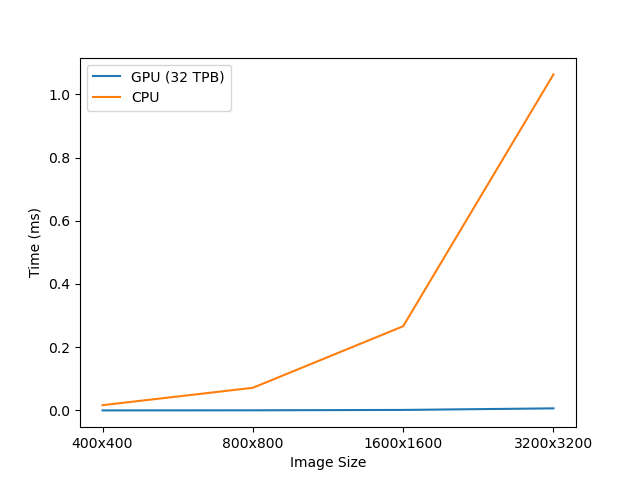
\includegraphics[scale=0.6]{plot2.png}
\end{center}

\ \\
\noindent
The results are clear from the first glance. It seems that the GPU times remain constant, while the CPU times skyrocket linearly with the increase in image size. For the next experiment, I have chosen to take another experiment, where I fix the size of the image to 1600x1600, but increase the size of the object linearly from 1.0 radius to 1.5, with a 0.1 step.
\begin{figure}[H]
    \centering
    \textbf{GPU rendering}\par\medskip
    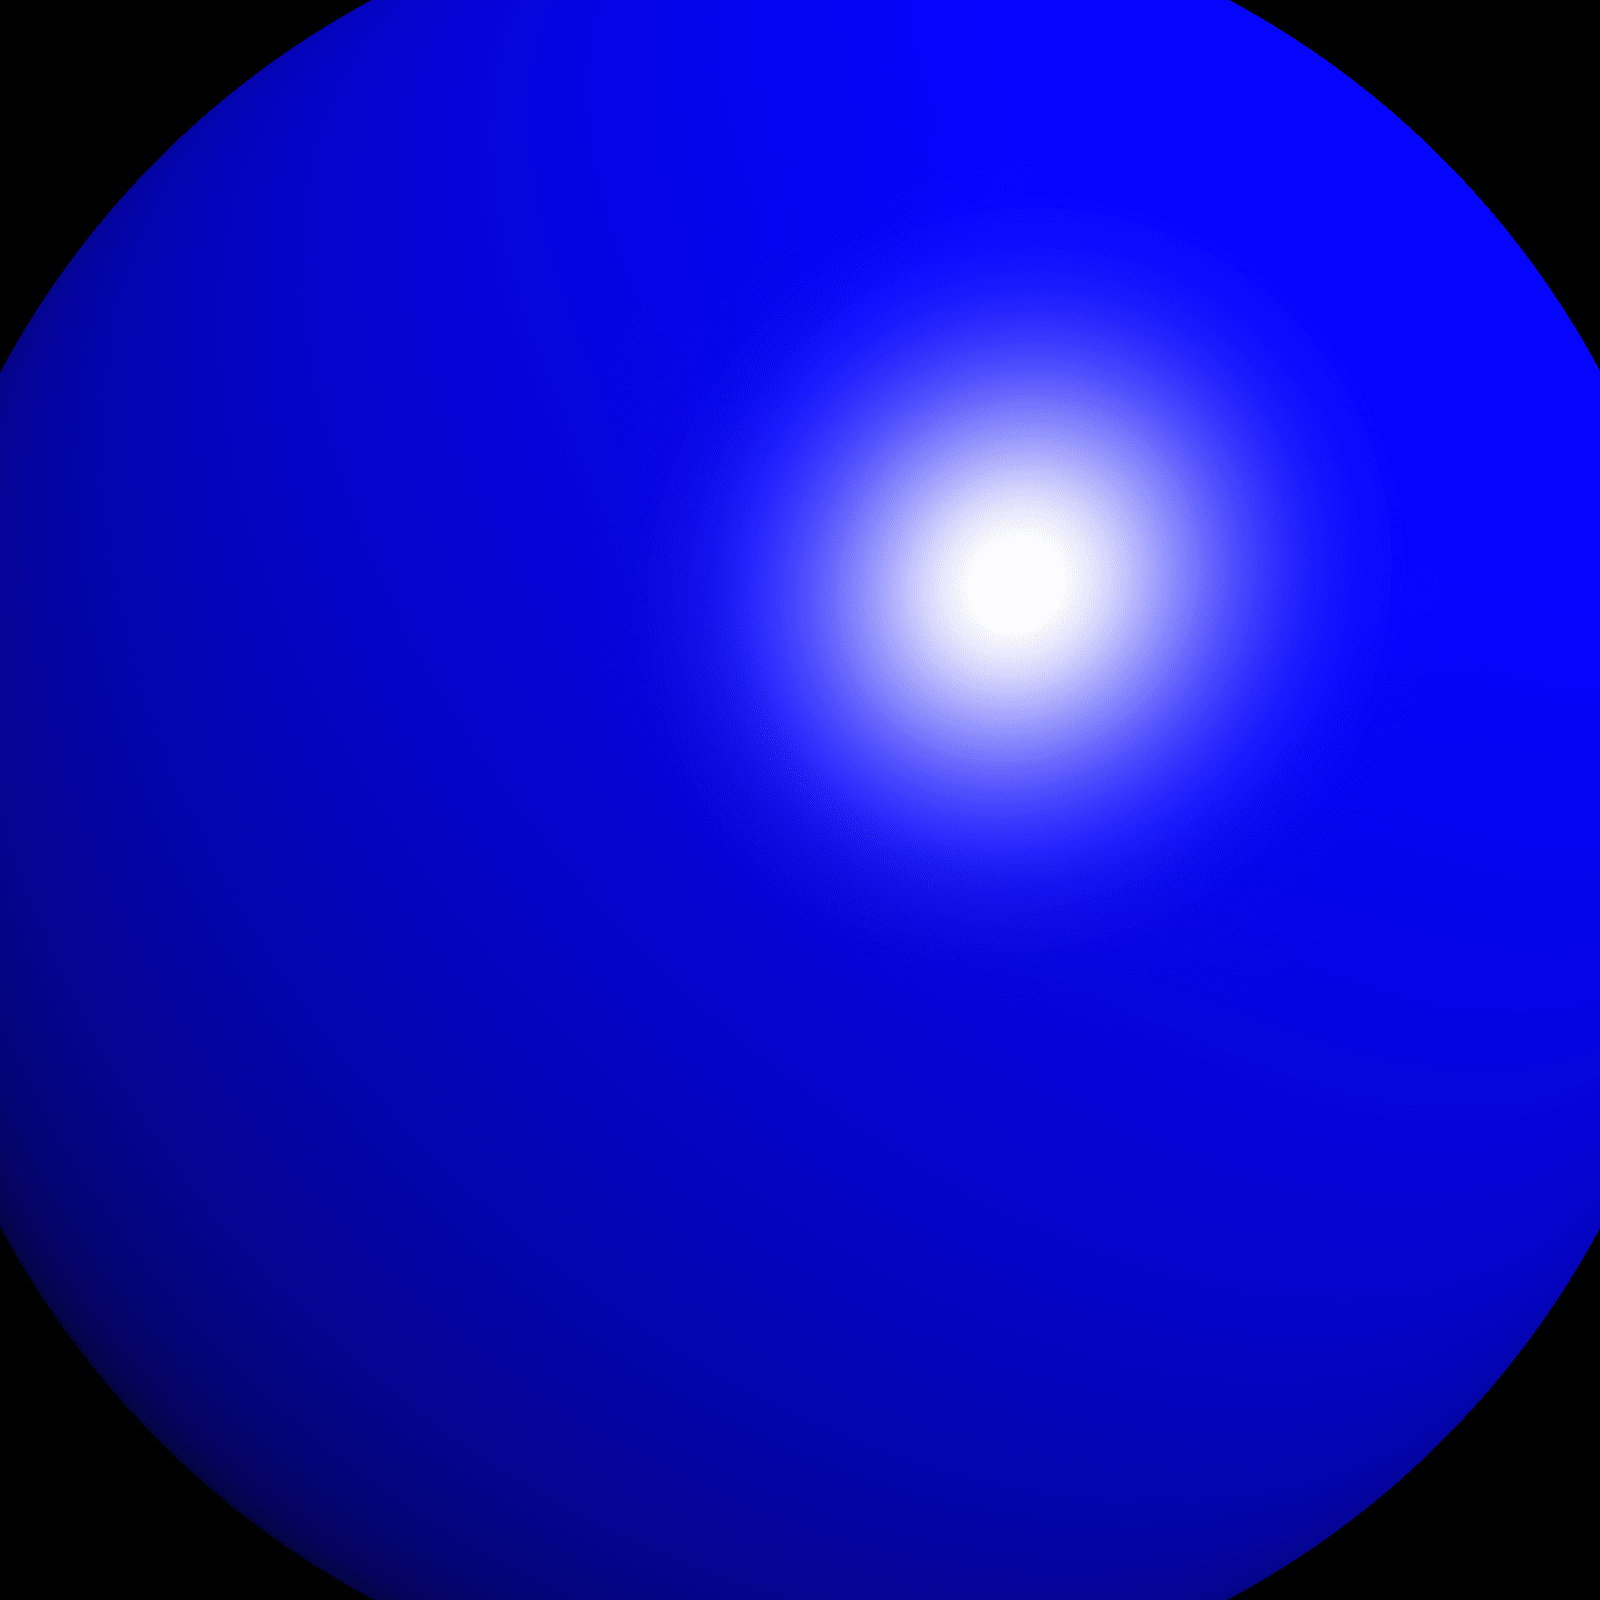
\includegraphics[scale=0.4]{gpu2.png}
    \caption{}
\end{figure}

\ \\
\noindent
If we try to increase the size of the object gradually and then compare the CPU and the GPU performance, we might find out that there is a significant increase in time with the CPU version, while the GPU tends to be linear, once again, the results are in Appendix \ref{tab:3}:

\begin{center}
  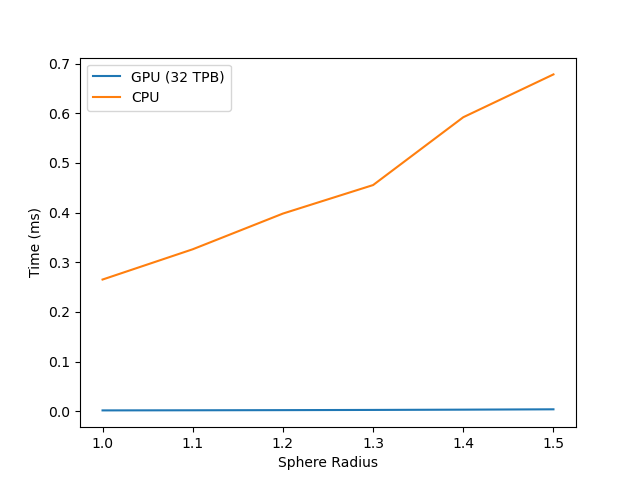
\includegraphics[scale=0.6]{plot3.png}
\end{center}

\clearpage
\ \\
\noindent
Finally, all the results from above show that the GPU outperforms the CPU in any of the cases, which is expected. Having a look at the results of running $nsys$ on the program (since $nvprof$ is no longer available for this platform), one can see that most of the time is spent actually on the $cudaMalloc$ functions and that the only memory copying is done from the device to the host, which we know from the code already: \\

\begin{lstlisting}[style=CStyle]
CUDA API Statistics:

 Time(%)  Total Time (ns)  Num Calls  Average (ns)  Minimum (ns)  Maximum (ns)  StdDev (ns)          Name         
 -------  ---------------  ---------  ------------  ------------  ------------  -----------  ---------------------
    94.6       95,379,771          1  95,379,771.0    95,379,771    95,379,771          0.0  cudaMalloc           
     3.5        3,528,058          1   3,528,058.0     3,528,058     3,528,058          0.0  cudaDeviceSynchronize
     1.8        1,840,779          1   1,840,779.0     1,840,779     1,840,779          0.0  cudaMemcpy           
     0.1          108,160          1     108,160.0       108,160       108,160          0.0  cudaFree             
     0.0           18,720          1      18,720.0        18,720        18,720          0.0  cudaLaunchKernel     



CUDA Kernel Statistics:

 Time(%)  Total Time (ns)  Instances  Average (ns)  Minimum (ns)  Maximum (ns)  StdDev (ns)      Name    
 -------  ---------------  ---------  ------------  ------------  ------------  -----------  ------------
   100.0        3,526,398          1   3,526,398.0     3,526,398     3,526,398          0.0  _Z7run_gpuPc



CUDA Memory Operation Statistics (by time):

 Time(%)  Total Time (ns)  Count  Average (ns)  Minimum (ns)  Maximum (ns)  StdDev (ns)      Operation     
 -------  ---------------  -----  ------------  ------------  ------------  -----------  ------------------
   100.0        1,521,443      1   1,521,443.0     1,521,443     1,521,443          0.0  [CUDA memcpy DtoH]



CUDA Memory Operation Statistics (by size):

 Total (MB)  Count  Average (MB)  Minimum (MB)  Maximum (MB)  StdDev (MB)      Operation     
 ----------  -----  ------------  ------------  ------------  -----------  ------------------
      7.680      1         7.680         7.680         7.680        0.000  [CUDA memcpy DtoH]
\end{lstlisting}

\section*{Discussion and Conclusion}

Overall, the assignment was really interesting and the visual results are always pleasing, since one can quantify the result of their experiment.\\
The results of the experiment are as expected, which means that the device (GPU) outperforms the host (CPU) in all of the tests. I ran some tests in order to find out which configuration would be the best and continued to use that for the rest of the experiments.
\\\\
One really important topic of discussion I think, and of reflection for myself is the topic of memory allocation in device kernels. So far, I have been allocating memory with the function $malloc$ on the device, which I have read through forums and documentation that is completely allowed and would work just fine. However, after some experimentation, it seems as if $malloc$ does not properly allocate memory on the device, since in all of the previous experiments, if one uses $malloc$ on the device, the times of the GPU are always a tiny bit worse than the times on the CPU. However, I could not find valuable documentation on this.

\clearpage


\bibliographystyle{myIEEEtran}
\renewcommand{\bibname}{References}
\addcontentsline{toc}{chapter}{References}
\bibliography{references}

\ \\ \ \\ \ \\

\section*{Appendix}

\subsection*{Table 1}
\begin{table}[H]
  \centering
  \begin{tabular}{ |p{4cm}||p{4cm}|p{4cm}|  }
    \hline
    \multicolumn{3}{|c|}{GPU times} \\
    \hline
    Time (seconds)& Image size& TPB (Threads per block)\\
    \hline
    0.001578& 400x400& 2\\
    0.000804& 400x400& 4\\
    0.000414& 400x400& 8\\
    0.000221& 400x400& 16\\
    \textbf{0.000128}& 400x400& 32\\
    0.000133& 400x400& 64\\
    0.000140& 400x400& 128\\
    0.000135& 400x400& 256\\
    0.006497& 800x800& 2\\
    0.003138& 800x800& 4\\
    0.001590& 800x800& 8\\
    0.000815& 800x800& 16\\
    \textbf{0.000424}& 800x800& 32\\
    0.000431& 800x800& 64\\
    0.000436& 800x800& 128\\
    0.000433& 800x800& 256\\
    0.026288& 1600x1600& 2\\
    0.013008& 1600x1600& 4\\
    0.006785& 1600x1600& 8\\
    0.003426& 1600x1600& 16\\
    0.001774& 1600x1600& 32\\
    \textbf{0.001621}& 1600x1600& 64\\
    0.001627& 1600x1600& 128\\
    0.001622& 1600x1600& 256\\
    \hline
  \end{tabular}
  \caption{Different Image sizes and TPB}
  \label{tab:1}
\end{table}


\subsection*{Table 2}
\begin{table}[H]
  \centering
  \begin{tabular}{ |p{4cm}||p{4cm}|p{4cm}|  }
    \hline
    \multicolumn{3}{|c|}{GPU vs CPU times with variable image size} \\
    \hline
    Platform & Time (seconds)& Image size\\
    \hline
    CPU & 0.016652 & 400x400\\
    CPU & 0.071616 & 800x800\\
    CPU & 0.266327 & 1600x1600\\
    CPU & 1.062895 & 3200x3200\\
    GPU& 0.000428& 800x800\\
    GPU& 0.000129& 400x400\\
    GPU& 0.001619& 1600x1600\\
    GPU& 0.006593& 3200x3200\\
    \hline
  \end{tabular}
  \caption{Different image sizes for CPU and GPU}
  \label{tab:2}
\end{table}

\subsection*{Table 3}
\begin{table}[H]
  \centering
  \begin{tabular}{ |p{4cm}||p{4cm}|p{4cm}|  }
    \hline
    \multicolumn{3}{|c|}{GPU vs CPU times with variable object radius} \\
    \hline
    Platform & Time (seconds)& Object Radius\\
    \hline
    GPU& 0.001615& 1.0\\
    GPU& 0.001856& 1.1\\
    GPU& 0.002155& 1.2\\
    GPU& 0.002560& 1.3\\
    GPU& 0.003112& 1.4\\
    GPU& 0.003804& 1.5\\
    
    CPU& 0.265073& 1.0\\
    CPU& 0.326033& 1.1\\    
    CPU& 0.397898& 1.2\\
    CPU& 0.455299& 1.3\\
    CPU& 0.591881& 1.4\\
    CPU& 0.678103& 1.5\\
    \hline
  \end{tabular}
  \caption{Different radius for the object rendered}
  \label{tab:3}
\end{table}



\end{document}
